\documentclass[a4paper]{article}
\usepackage{tikz}
\usepackage{geometry}
\usepackage{graphicx}
\usepackage{natbib}
\usepackage{amsmath}
\usepackage{amssymb}
\usepackage{amsthm}
\usepackage{paralist}
\usepackage{epstopdf}
\usepackage{tabularx}
\usepackage{longtable}
\usepackage{multirow}
\usepackage{multicol}
\usepackage[hidelinks]{hyperref}
\usepackage{fancyvrb}
\usepackage{algorithm}
\usepackage{algorithmic}
\usepackage{float}
\usepackage{paralist}
%\usepackage[svgname]{xcolor}
\usepackage{enumerate}
\usepackage{array}
\usepackage{times}
\usepackage{url}
\usepackage{fancyhdr}
\usepackage{comment}
\usepackage{environ}
\usepackage{times}
\usepackage{textcomp}
\usepackage{caption}
\usepackage{bbm}


\urlstyle{rm}

\setlength\parindent{0pt} % Removes all indentation from paragraphs
\theoremstyle{definition}
\newtheorem{definition}{Definition}[]
\newtheorem{conjecture}{Conjecture}[]
\newtheorem{example}{Example}[]
\newtheorem{theorem}{Theorem}[]
\newtheorem{lemma}{Lemma}
\newtheorem{proposition}{Proposition}
\newtheorem{corollary}{Corollary}

\floatname{algorithm}{Procedure}
\renewcommand{\algorithmicrequire}{\textbf{Input:}}
\renewcommand{\algorithmicensure}{\textbf{Output:}}
\newcommand{\abs}[1]{\lvert#1\rvert}
\newcommand{\norm}[1]{\lVert#1\rVert}
\newcommand{\RR}{\mathbb{R}}
\newcommand{\CC}{\mathbb{C}}
\newcommand{\Nat}{\mathbb{N}}
\newcommand{\br}[1]{\{#1\}}
\DeclareMathOperator*{\argmin}{arg\,min}
\DeclareMathOperator*{\argmax}{arg\,max}
\renewcommand{\qedsymbol}{$\blacksquare$}

\definecolor{dkgreen}{rgb}{0,0.6,0}
\definecolor{gray}{rgb}{0.5,0.5,0.5}
\definecolor{mauve}{rgb}{0.58,0,0.82}

\definecolor{C0}{HTML}{1F77B4}
\definecolor{C1}{HTML}{FF7F0E}
\definecolor{C2}{HTML}{2ca02c}
\definecolor{C3}{HTML}{d62728}
\definecolor{C4}{HTML}{9467bd}
\definecolor{C5}{HTML}{8c564b}
\definecolor{C6}{HTML}{e377c2}
\definecolor{C7}{HTML}{7F7F7F}
\definecolor{C8}{HTML}{bcbd22}
\definecolor{C9}{HTML}{17BECF}

\newcommand{\Var}{\mathrm{Var}}
\newcommand{\Cov}{\mathrm{Cov}}
\newcommand{\sgn}{\mathrm{sgn}}

\newcommand{\vc}[1]{\boldsymbol{#1}}
\newcommand{\xv}{\vc{x}}
\newcommand{\Sigmav}{\vc{\Sigma}}
\newcommand{\alphav}{\vc{\alpha}}
\newcommand{\muv}{\vc{\mu}}

\newcommand{\red}[1]{\textcolor{red}{#1}}

\def\x{\mathbf x}
\def\y{\mathbf y}
\def\w{\mathbf w}
\def\v{\mathbf v}
\def\E{\mathbb E}
\def\R{\mathbb R}
\def\V{\mathbb V}
\def\ind{\mathbbm 1}

% TO SHOW SOLUTIONS, include following (else comment out):
\newenvironment{soln}{
    \leavevmode\color{blue}\ignorespaces
}{}


\hypersetup{
%    colorlinks,
    linkcolor={red!50!black},
    citecolor={blue!50!black},
    urlcolor={blue!80!black}
}

\geometry{
  top=1in,            % <-- you want to adjust this
  inner=1in,
  outer=1in,
  bottom=1in,
  headheight=3em,       % <-- and this
  headsep=2em,          % <-- and this
  footskip=3em,
}


\pagestyle{fancyplain}
\lhead{\fancyplain{}{Homework 7}}
\rhead{\fancyplain{}{CS 760 Machine Learning}}
\cfoot{\thepage}

\title{\textsc{Homework 7}} % Title

%%% NOTE:  Replace 'NAME HERE' etc., and delete any "\red{}" wrappers (so it won't show up as red)

\author{
$>>$Sean Sun$<<$ \\
$>>$9078202463$<<$\\
} 

\date{}

\begin{document}

\maketitle 


\textbf{Instructions:} 
Although this is a programming homework, you only need to hand in a pdf answer file.
There is no need to submit the latex source or any code.
You can choose any programming language, as long as you implement the algorithm from scratch.

Use this latex file as a template to develop your homework.
Submit your homework on time as a single pdf file to Canvas.
Please check Piazza for updates about the homework.


\section{VC dimension (30 pts)}
Let the input $x\in X=\R$.
Consider $F=\{f(x)=\sgn(ax^2+bx+c): a, b, c \in \R\}$, where $\sgn(z)=1$ if $z\ge0$, and 0 otherwise.
What is $VC(F)$?  Prove it.

\begin{soln}
$VC(F) = 3$\\
Proof:
\\When there are 4 points, $F$ can not satisfy the binary vectore of [0, 1, 0, 1] or [1, 0, 1, 0]. So, $F$ can't shatter a set with 4 points. 
\\When there are more than 4 points, for every contiguous four elements in the binary vecter, $F$ still can't satisfy the binary vectore of [0, 1, 0, 1] or [1, 0, 1, 0]. So, $F$ can't shatter a set with more than 4 points.
\\So, $VC(F)$ = 3
\end{soln}


\section{Verify PAC Bound (30 pts)}
Let $h$ be the VC dimension of function family $F$.
For any $\delta>0$, with probability at least $1-\delta$ we have
$$R(\hat f_S) - \hat R_S(\hat f_S) \le 2 \sqrt{2 \frac{h \log n + h \log\frac{2e}{h}  + \log \frac{2}{\delta} }{n}},$$
where $R(f) = \E 1_{[f(x)\neq y]}$ is the risk of $f$,
$S=(x_1,y_1), \ldots, (x_n, y_n)$ is a training set of size $n$,
$\hat R_S(f) = {1\over n} \sum_{i=1}^n 1_{[f(x_i)\neq y_i]}$ is the empirical risk of $f$ on $S$,
and 
$\hat f_S \in \argmin_{f\in F} \hat R_S(f)$ is an empirical risk minimizer (ERM).

We now verify this bound on a simple classification task.  Let $p(x)=\mathrm{uniform}([-1,1])$.  Given $x$, the label is deterministic: $y=\sgn(x)$.
Recall $\sgn(x)=1$ if $x\ge 0$, and 0 otherwise.
This means the true decision boundary is at $x=0$.
Let $f_\theta(x) := \sgn(x-\theta)$ which has threshold at $\theta$.
Let $F=\{f_\theta: \theta \in [-1,1]\}$.  
\begin{enumerate}
\item Given $S$, find the smallest positive item: $a = \min_{(x_i, y_i)\in S: y_i=1} x_i$ if one exists, otherwise let $a=1$.  Is $\hat f_S := f_a$ an ERM?  Justify your answer.

\begin{soln}
$\hat f_S := f_a$ is an ERM.\\
When there are positive $x_i$s, every $x_j > \min_{(x_i, y_i)\in S: y_i=1} x_i$ where $((x_j, y_j)\in S)$ will be labeled as 1 and all other points will be labeled as 0. So, setting the threshold at $ \min_{(x_i, y_i)\in S: y_i=1} x_i$ will lead to zero empirical risk.
\\When there are no positive $x_i$, all points will be labeled as 0, so setting the threshold at 1 will label all points to be 0 and thus leads to zero empirical risk.
\\ So, $\hat f_S := f_a$ is an ERM.
\end{soln}

\item Derive $R(f_a)$.

\begin{soln}
$R(f_a) = 1\times p( a > x \ge 0 ) = \frac {a} {2}$
\end{soln}

\item Derive $\hat R_S(f_a)$.

\begin{soln}
$\hat R_S(f_a) = 0$
\end{soln}

\item What is the VC dimension of $F$?  Note $F$ contains threshold classifiers of the type ``left negative, right positive.''

\begin{soln}
$VC(F) = 1$ \\
this one-sided threshold classifier can't satisfy the binary vector [1,0] because all points on the left of threshold will be labeled as 0 and all points on the right of threshold will be labeled as 1
\end{soln}
 
\item Fix $\delta=0.05$ (95\% confidence) and $n=200$.  Compute 
$2 \sqrt{2 \frac{h \log n + h \log\frac{2e}{h}  + \log \frac{2}{\delta} }{n}}.$
This is natural log.

\begin{soln}
$2 \sqrt{2 \frac{h \log n + h \log\frac{2e}{h}  + \log \frac{2}{\delta} }{n}} = 2 \sqrt{2 \frac{1 \log 200 + 1 \log\frac{2e}{1}  + \log \frac{2}{0.05} }{200}} = 2 \sqrt{ \frac{ \log 200 + log2 + 1 + \log 40}{100}} =  2 \sqrt{ \frac{ \log 16000 + 1}{100}} =0.654$
\end{soln}

\item Generate 10,000 random training sets from $p(x)$ and the associated labels.  Each training set $S$ has $n=200$ points.
On each $S$ you will compute $R(f_a) - \hat R_S(f_a)$.
Now you have 10,000 numbers. (1) Produce a histogram of them.  (2) Find the 95\% quantile of them.  (3) Compare the 95\% quantile to the bound in the previous question.  Discuss your observations.

\begin{soln}
(1)\\
\begin{center}
	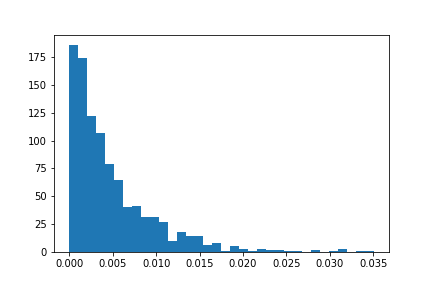
\includegraphics[width=4in]{q26}
\end{center}

(2)\\
The 95\% quantile is 0.01475

(3)\\
The bound with 95\% confidence from question 5 was 0.654, which is a much broader bound than 0.01475. So the bound we got from question 5 is acceptable.

\end{soln}


\end{enumerate}


\section{Q-learning (40 pts)}
Consider the following Markov Decision Process.
It has two states $s$.
It has two actions $a$: move and stay.
The state transition is deterministic: ``move'' moves to the other state, while ``stay' stays at the current state.
The reward $r$ is 0 for move,  1 for stay. 
There is a discounting factor $\gamma=0.9$.
\\
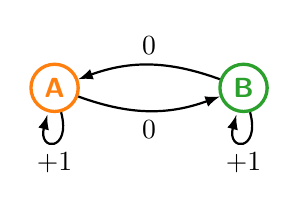
\begin{tikzpicture}
\tikzstyle{n} = [very thick,circle,inner sep=0mm,minimum width=6mm]
\tikzstyle{a} = [thick,>=latex,->]
\def\dx{1.2}
\def\dy{-1.2}
\node[n,C1,draw=C1] (2) at (\dy,0) {\textbf{\textsf{A}}};
\node[n,C2,draw=C2] (1) at (\dx,0) {\textbf{\textsf{B}}};
\path[a]
(2) edge [loop below] node {+1}(2)
(1) edge [loop below] node {+1}(1)
(2) edge [bend right=20] node[below] {0}(1)
(1) edge [bend right=20] node[above] {0}(2);
\end{tikzpicture}

The reinforcement learning agent performs Q-learning.  Recall the $Q$ table has entries $Q(s,a)$.
The $Q$ table is initialized with all zeros.
The agent starts in state $s_1=A$.
In any state $s_t$, the agent chooses the action $a_t$ according to a behavior policy $a_t = \pi_B(s_t)$.
Upon experiencing the next state and reward $s_{t+1}, r_t$ the update is:
$$Q(s_t, a_t) \Leftarrow (1-\alpha) Q(s_t, a_t) + \alpha \left( r_t + \gamma \max_{a'} Q(s_{t+1}, a') \right).$$
Let the step size parameter $\alpha=0.5$.

\begin{enumerate}
\item Run Q-learning for 200 steps with a uniformly random behavior policy: $\pi_B(s_t)=$ move or stay with 1/2 probability for any $s_t$.
Show the Q table at the end.

\begin{soln}

\begin{center}
\begin{tabular}{ |c|c|c| } 
 \hline
  & stay& move \\ 
 \hline
 A & 9.48078 & 7.99048 \\ 
 \hline
B & 9.00271& 8.29473\\ 
 \hline
\end{tabular}
\end{center}

\end{soln}

\item Reset and repeat the above, but with an $\epsilon$-greedy behavior policy: at each state $s_t$, with probability $1-\epsilon$ choose what the current Q table says is the best action: $\argmax_a Q(s_t,a)$; Break ties arbitrarily. Otherwise (with probability $\epsilon$) uniformly chooses between move and stay.
Use $\epsilon=0.5$.

\begin{soln}

\begin{center}
\begin{tabular}{ |c|c|c| } 
 \hline
  & stay& move \\ 
 \hline
 A & 9.82054 & 8.69072 \\ 
 \hline
B & 9.73766& 8.79053\\ 
 \hline
\end{tabular}
\end{center}

\end{soln}

\item Reset and repeat the above, but with a deterministic greedy behavior policy: at each state $s_t$ use the best action $a_t \in \argmax_a Q(s_t,a)$ indicated by the current Q table. If there is a tie, prefer move.

\begin{soln}

\begin{center}
\begin{tabular}{ |c|c|c| } 
 \hline
  & stay& move \\ 
 \hline
 A & 0 & 0 \\ 
 \hline
B & 0& 0\\ 
 \hline
\end{tabular}
\end{center}

\end{soln}

\item Without doing simulation, use Bellman equation to derive the true Q table induced by the MDP.
\begin{soln}
$V*(s) = E[r(s,\pi*(s)] + \gamma E_{s' |(s, \pi*(s))} [V*(s')] = 1 + 0.9\times V*(s)$\\  
So, $V*(s) = 10$
$Q(s, move) = E[r(s, move)] + \gamma E_{s' |s, move}[V*(s')] = 0 + 0.9\times 10 = 9$\\
$Q(s, stay) = E[r(s, stay)] + \gamma E_{s' |s, stay}[V*(s')] = 1 + 0.9\times 10 = 10$\\

\begin{center}
\begin{tabular}{ |c|c|c| } 
 \hline
  & stay& move \\ 
 \hline
 A & 10 & 9 \\ 
 \hline
B & 10& 9\\ 
 \hline
\end{tabular}
\end{center}

\end{soln}


\end{enumerate}


\end{document}
